\begin{SCfigure}[][p]
    \centering
    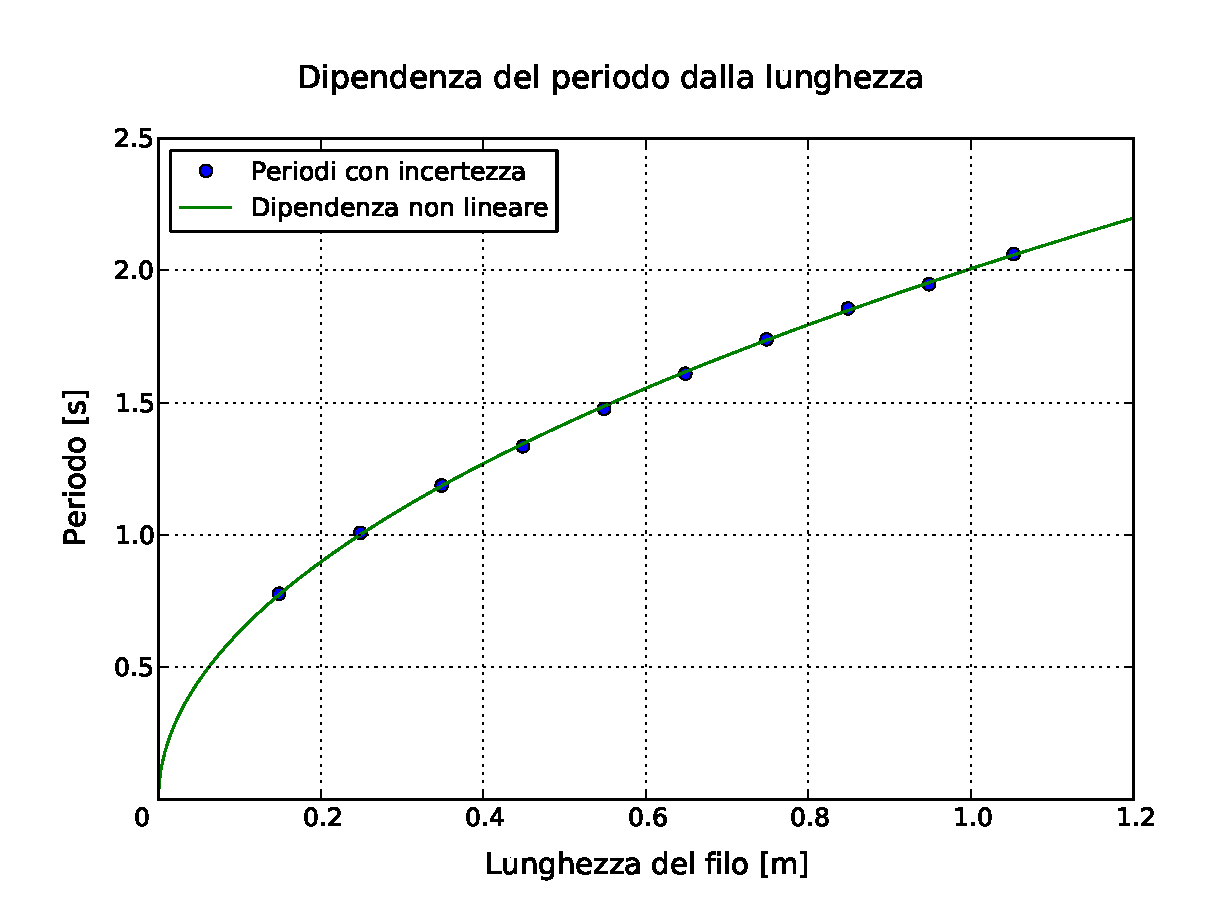
\includegraphics[width=120mm]{immagini/lunghezza_periodo.pdf}
    \caption{Il grafico in figura mostra il periodo del pendolo in funzione della lunghezza del filo.
        Le barre di errore non sono mostrate in quanto sono dell'ordine di grandezza dei punti. Si
        nota immediatamente l'andamento non lineare dei dati sperimentali. La curva in
        figura è la funzione $\mathcal{T} = a\ell^b$ con i valori di $a$ e $b$ calcolati con la regressione
        nel paragrafo \ref{l_regressione}.}
    \label{fig:lunghezza_periodo}
\end{SCfigure}

\begin{SCfigure}[][p]
    \centering
    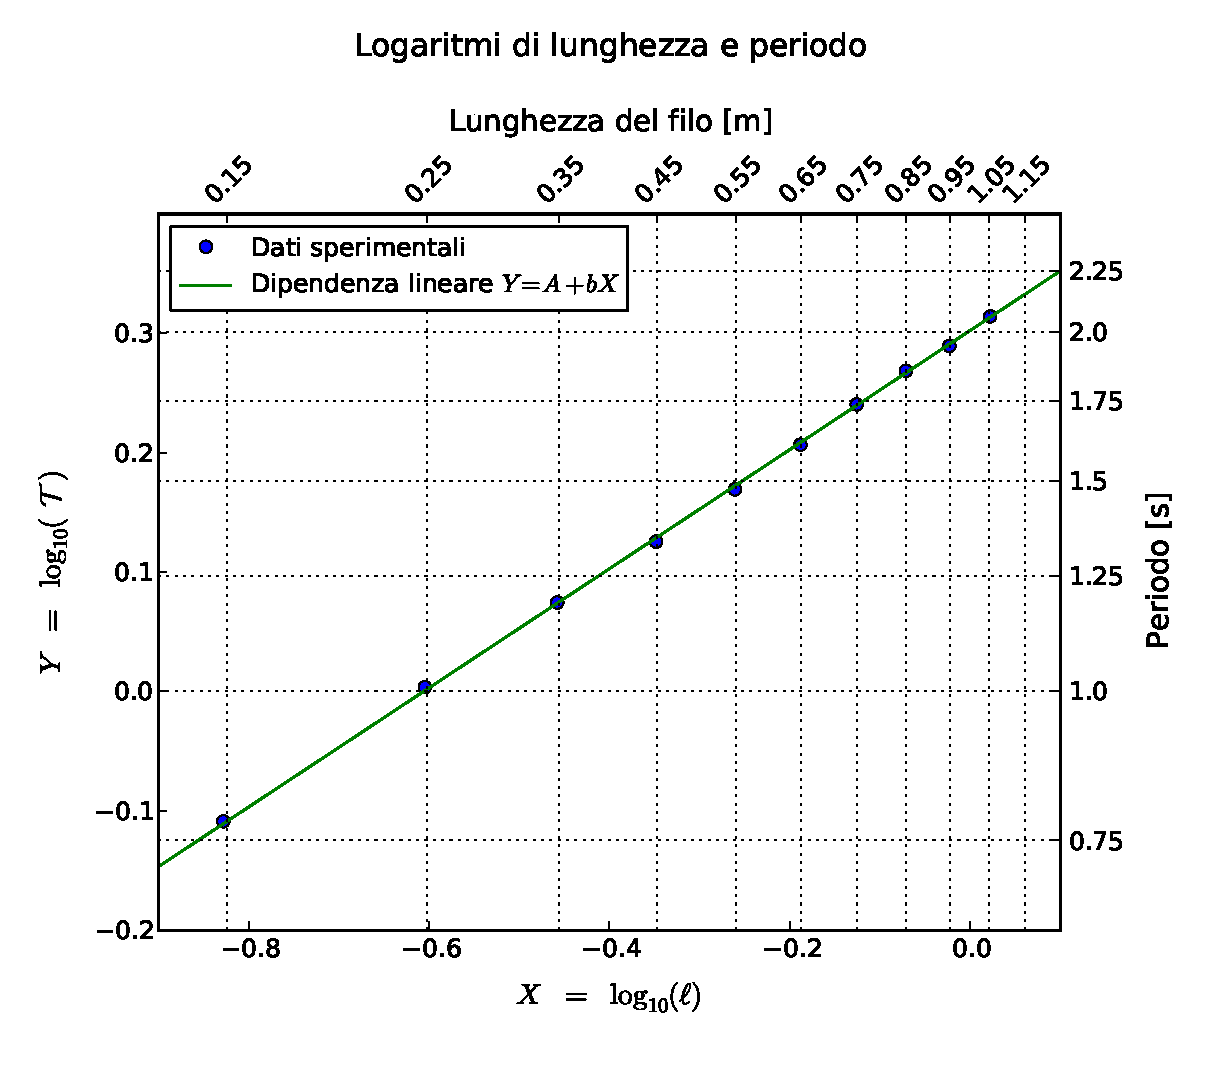
\includegraphics[width=120mm]{immagini/log.pdf}
    \caption{Il grafico è analogo a quello nella figura \ref{fig:lunghezza_periodo}, con la sola differenza
        che in questo caso si tratta di un plot $X = \log_{10} (\ell)$ versus $Y = \log_{10} (\mathcal{T})$, o, equivamentemente,
        gli assi sono in scala logaritmica. Le barre d'errore non sono mostrate poiché invisibili a questa scala.
        In questo grafico si nota la relazione lineare tra $X$ e $Y$, rappresentata dalla retta $Y = A + bX$, con $A$ e $b$ calcolati
    mediante regressione. Notare che $X$ e $Y$ sono numeri puri poichè si fa il logaritmo dei soli valori numerici di $\ell$ e $\mathcal{T}$.}
    \label{fig:lunghezza_periodo_log}
\end{SCfigure}

\label{l_pred_teo}

Graficando i dati ottenuti nel paragrafo precedente, ci si accorge immediatamente (si veda
la figura \ref{fig:lunghezza_periodo}) che il periodo del pendolo dipende dalla lunghezza
del suo filo, come correttamente previsto dalla teoria. Tuttavia la dipendenza è chiaramente non lineare.

Dall'espressione (\ref{eq:periodo_pendolo}) per il periodo del pendolo semplice, si sa che
il periodo vale

\begin{equation}
    \mathcal{T} = 2\pi\sqrt{\frac{\ell}{g}}
    \tag{\ref{eq:periodo_pendolo}}
\end{equation}

Tuttavia qui assumiamo come ipotesi una dipendenza del tipo:

\begin{equation}
    \mathcal{T} = a\ell^b
    \label{eq:ipotesi}
\end{equation}
%
dove $a$ e $b$ sono due costanti\footnote{$b$ è adimensionale, mentre $a$ deve avere dimensioni [$\text{s}\,\text{m}^{-b}$] affinché le unità di misura l'equazione (\ref{eq:ipotesi}) siano corrette}.
Dal grafico in figura \ref{fig:lunghezza_periodo} si può intuire una dipendenza di questo genere.
Confrontando l'equazione (\ref{eq:periodo_pendolo}) con la (\ref{eq:ipotesi}) otteniamo che, secondo il modello
del pendolo semplice, deve valere

\begin{equation}
    a = \frac{2\pi}{\sqrt{g}} \; \frac{\text{s}}{\sqrt{\text{m}}} = 2.006 \qquad \qquad b = \frac{1}{2}
\end{equation}
%
dove per il calcolo di $a$ abbiamo utilizzato il valore $g = \SI{9.806}{\meter\per\square\second}$, di cui trascuriamo l'incertezza
(si veda la sottosezione \ref{g_confronto} ed in particolare l'equazione (\ref{eq:g_f})).

Queste sono le predizioni teoriche del modello del pendolo semplice. Calcolando $a$ e $b$ dai dati sperimentali
possiamo quindi verificare la correttezza della formula (\ref{eq:periodo_pendolo}).

Vogliamo ora linearizzare l'equazione (\ref{eq:ipotesi}) per poter utilizzare la regressione lineare e ricavare $a$ e $b$.
Al tal fine, definiamo due nuove variabili\footnote{Da notare che $X$ e $Y$, e di conseguenza le loro incertezze,
sono grandezze adimensionali poiché
le funzioni trascendenti, come il logaritmo, hanno argomenti e valori adimensionali. Nella relazione viene sottinteso
che i valori $\ell$ e $\mathcal{T}$, quando sono argomento di logaritmi, indicano solo il valore numerico e non la grandezza fisica
\emph{lunghezza del filo} o \emph{periodo del pendolo}.}:

\begin{equation}
    X := \log_{10}{(\ell)} \qquad \qquad Y := \log_{10}{(\mathcal{T})}
    \label{eq:vars}
\end{equation}

Le incertezze su $X$ e $Y$, calcolate con la regola di propagazione, sono

\begin{equation}
    \delta X = \frac{\log_{10}(e)}{\ell}\delta \ell
    \qquad \qquad
    \delta Y = \frac{\log_{10}(e)}{\mathcal{T}}\delta\mathcal{T}
    \label{eq:delta_XY}
\end{equation}

Quindi, applicando ad entrambi i membri della (\ref{eq:ipotesi}) il logaritmo, si ottiene\footnote{
Anche $A$ è adimensionale.}

\begin{equation}
    Y = \log_{10} (\mathcal{T}) = \log_{10} (a) + b \log_{10} (\ell) = A + b X
\end{equation}
%
dove $A := \log_{10} a$ e dunque $a = 10^A$. La legge trovata è lineare, come mostrato dal grafico
in Figura \ref{fig:lunghezza_periodo_log}, e si può quindi utilizzare la consueta procedura di fit.

%\begin{table}
%    \centering
%    \begin{tabular}{c c c c}
%    \end{tabular}
%\end{table}

\subsubsection{Regressione}
\label{l_regressione}

Per cominciare abbiamo calcolato, per ogni coppia ($\ell_i$, $\mathcal{T}_i$), i valori $X_i$ e $Y_i$
e le relative incertezze $\delta X_i$ e $\delta Y_i$, usando le formule (\ref{eq:vars}) e (\ref{eq:delta_XY}).

Procediamo ora con il calcolo dei parametri A e b tramite regressione lineare. 
La regressione si basa sulla minimizzazione della funzione

\begin{equation}
    \sum_{i=1}^\mathcal{N} \frac{(Y_i - A - bX_i)^2}{(\delta Y_i^{\text{tot}})^2}
    \qquad \qquad \text{dove} \quad
    \delta Y_i^{\text{tot}} = \sqrt{\delta Y_i^2 + b^2 \delta X_i^2}
    \label{eq:min_quad}
\end{equation}
%
dove $\mathcal{N} = 10$ indica il numero di lunghezze testare.

Questa funzione misura la discrepanza tra legge lineare e dati sperimentali. Minimizzando la (\ref{eq:min_quad}) si ottengono
i valori di $A$ e $b$, ovvero la retta, che interpretano in modo ``migliore'' i dati.

Come prima cosa si è stimato il parametro b per trasferire l'incertezza dalle X alle Y.
La stima è stata ottenuta ignorando l'incertezza sulle X, ovvero ponendo $\delta Y_i^{\text{tot}} = \delta Y_i$ e facendo un fit preliminare.
Dai calcoli risulta:

\begin{equation}
    b' + \delta b' = 0.499 \pm 0.002
\end{equation}

Abbiamo utilizzato questo valore $b'$ per trasferire l'incertezza e calcolare $\delta Y_i^{\text{tot}}$. Minimizzando nuovamente la 
(\ref{eq:min_quad}) con i nuovi valori dell'incertezza trovati, si ha che:

\begin{equation}
    A = 0.3024 \qquad \qquad b = 0.499
\end{equation}

Le incertezze su $A$ e $b$ si possono ricavare con la propagazione dell'incertezza e valgono:

\begin{equation}
    \delta A = 0.0005 \qquad \qquad \delta b = 0.002
\end{equation}

Prima di proseguire notiamo che il valore di $b$ ricavato dalla regressione è compatibile con la stima $b'$
ricavata dal fit preliminare, in quanto i risultati sono uguali entro l'incertezza. Questo indica anche che
l'incertezza trasferita dalle $X$ è trascurabile rispetto all'incertezza sulle $Y$.
